\subsection{Circuito Driver}

Como se explicó más arriba, para excitar un transistor MOSFET y encenderlo, es necesario mantener una tensión $V_{GS}$ entre gate y source mayor a una tensión umbral dependiente del modelo. En nuestro caso, esta tensión umbral del IRFP150N es de \SI[]{4}[]{\volt}, como se ve en la tabla \ref{tabla:IRFP150}. Entonces, se debe diseñar algún circuito que sea capaz de proveer estos pulsos de tensión al gate de cada transistor, entregando también la corriente necesaria para cargar y descargar sus capacitancias de gate suficientemente rápido (llamadas corrientes de \textit{source} y \textit{sink}).\\

Este es el llamado {\Medium circuito \textit{driver}} o {\Medium circuito de excitación} y debe existir uno para cada uno de los cuatro transistores del puente. Ahora debemos establecer algunos requerimientos que debe cumplir el circuito:\\

\begin{itemize}
    \item Tensión de operación mayor a \SI[]{100}[]{\volt}, por encima de la máxima tensión de la pila de combustible.
    \item Tiempos de encendido y apagado mucho menores al período $T_s$ de \SI[]{50}[]{\micro\second} de la excitación.
    \item Corrientes de sink y source mayores a \SI[]{2}[]{\ampere} para cargar rápidamente las capacitancias de los transistores, calculado según la nota de aplicación de \cite{SinkSourceCurrent}.
    \item Se busca utilizar una solución integrada, ya que suelen ser más compactas y sencillas.
    \item Es deseable el uso de componentes de montaje superficial o SMD.\\
\end{itemize}

Con estos datos vamos a seleccionar y diseñar un circuito de excitación y explicar brevemente el funcionamiento de todas sus partes.\\

\subsubsection{Selección y Diseño}

Existen diversos tipos de soluciones integradas para circuitos de excitación de transistores MOSFET. Se pueden encontrar circuitos de uno o múltiples canales; existen circuitos que incluyen una aislación entre las entradas y salidas; entre otras funcionalidades. También se consiguen con distintas funciones de seguridad y protección, como el \textit{dead-time}, que permite forzar un tiempo fijo entre la activación de dos transistores de la misma rama, evitando situaciones de cortocircuito; y el \textit{undervoltage lockout} (UVLO), que evita daños por condiciones de baja tensión.\\

Entre todas las opciones, originalmente se había decidido por el modelo UCC21540 de Texas Instruments, un driver de doble canal, con aislación incluida, funcionalidades de dead-time y UVLO, alta capacidad de corriente y un encapsulado SMD de tipo SOIC-16.\\

Sin embargo, este dispositivo no se pudo obtener por falta de disponibilidad, por lo que se tuvo que buscar una alternativa de características similares que esté en disponibilidad. Se terminó decidiendo por el integrado {\Medium 2ED21834-S06J de Infineon Technologies}, cuyas especificaciones básicas se muestran a continuación.\\

\setlength{\tabcolsep}{7pt}
\renewcommand{\arraystretch}{1.5}
\begin{table}[h]
\begin{center}
    \begin{tabular}{llrrrr}
    {\SemiBold Fabricante} & {\SemiBold Modelo} & $\mathbf{V_S}$ [\unit{\volt}] & $\mathbf{I_{OH}/\mathbf{I_{OL}}}$ [\unit{\ampere}] & $\mathbf{t_{on}}/\mathbf{t_{off}}$ [\unit{\nano\second}] & $\mathbf{V_{cc}}$ [\unit{\volt}]\\
    \hline
    Infineon & 2ED21834-S06J & \num{650} & \num{2.5} & \num{200} & \num{10}-\num{20}
    \end{tabular}
    \caption{Especificaciones del driver modelo 2ED21834-S06J de Infineon Technologies.\textsuperscript{\cite{DatasheetDriver}}}
    \label{tabla:driver}
\end{center}
\end{table}

Donde $V_S$ es la máxima tensión común de operación, $I_{OH}$ e $I_{OL}$ son las corrientes máximas de source y sink, $t_{on}$ y $t_{off}$ son los tiempos de encendido y apagado, y $V_{cc}$ es el rango de tensiones de alimentación.\\ 

El 2ED21834-S06J es un driver de doble canal para medios puentes de transistores de tipo MOSFET e IGBT, con diodo y resistencia de bootstrap incluidos además de funcionalidad de dead-time y UVLO para circuitos del lado bajo y alto, todo contenido en un encapsulado SMD de catorce pines del tipo DSO-14 (figura \ref{encapsulado_driver}). Sus corrientes sink y source de \SI[]{2.5}[]{\ampere} superan la corriente necesaria calculada para los IRFP150N de la tabla \ref{tabla:IRFP150}, su tensión de operación se encuentra cómodamente por encima de la tensión de operación del primario del convertidor, además de tener muy bajos tiempos de conmutación.\\

\begin{figure}[h]
    \centering
    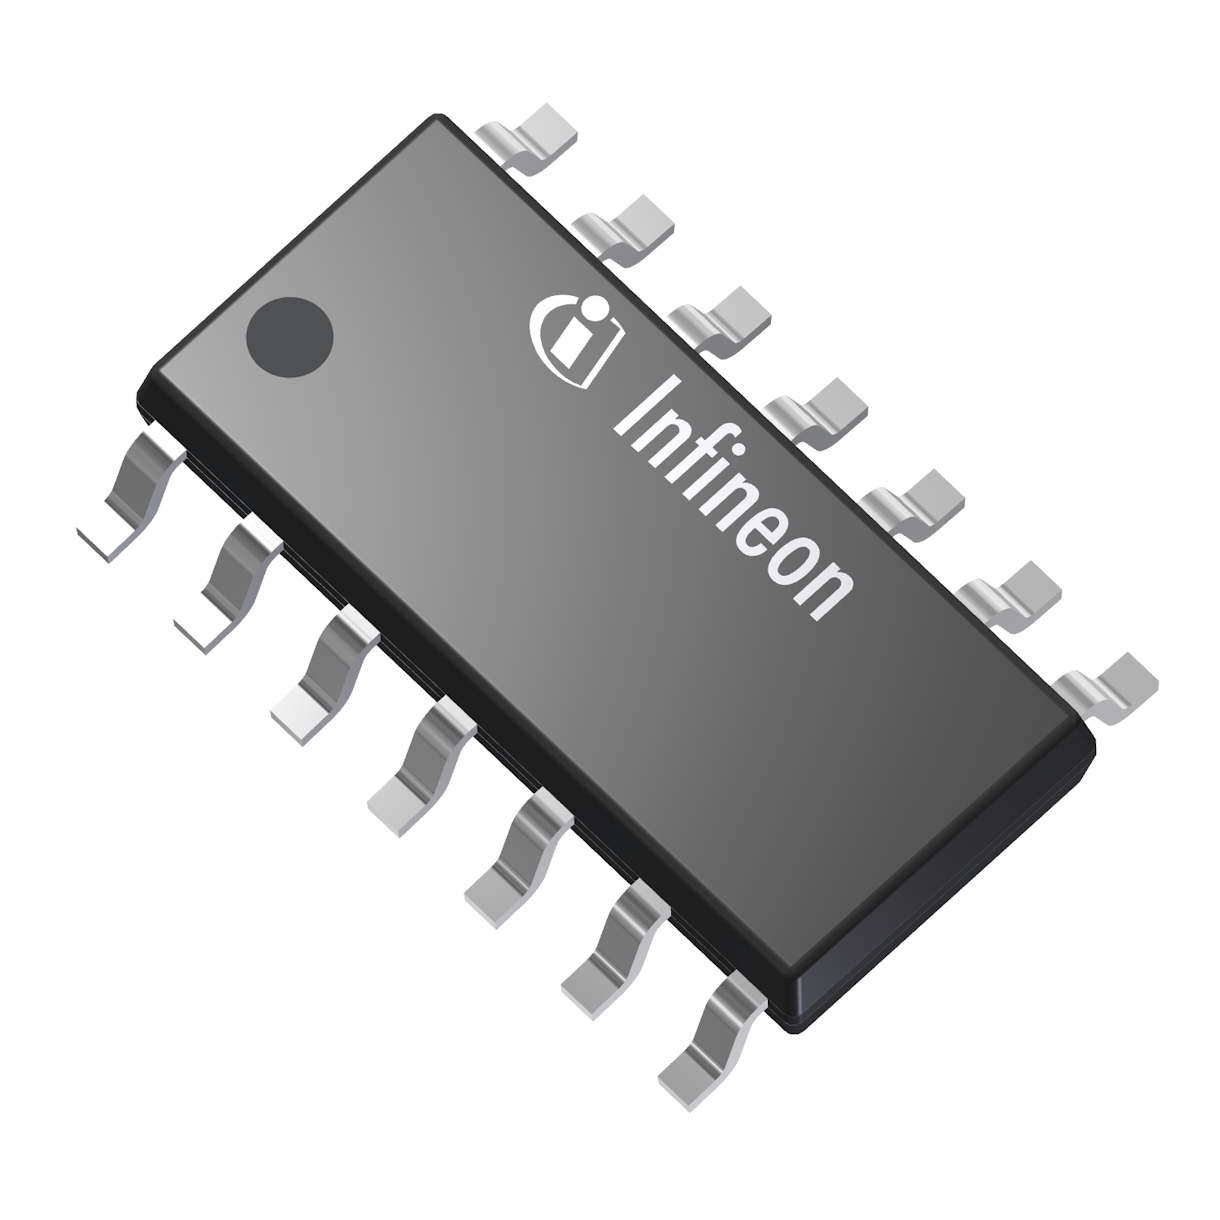
\includegraphics[scale=0.07]{Imagenes/Driver DSO-14.png}
    \caption{Driver 2ED21834-S06J con su encapsulado SMD tipo DSO-14.}
    \label{encapsulado_driver}
\end{figure}

En nuestro caso, se deben utilizar dos de estos dispositivos, uno para cada columna del puente completo. Vamos a utilizar la función de dead-time, configurable mediante una resistencia conectada al pin DT, para proteger contra posibles cortocircuitos causados por la activación errónea de ambos transistores de una columna simultáneamente (\textit{shoot-through}). El resto de la conexión de componentes del driver se realizó de acuerdo a las recomendaciones del fabricante encontradas en la hoja de datos \cite{DatasheetDriver}, que se puede ver en la figura \ref{circuito_driver}.\\

\begin{figure}[h]
    \centering
    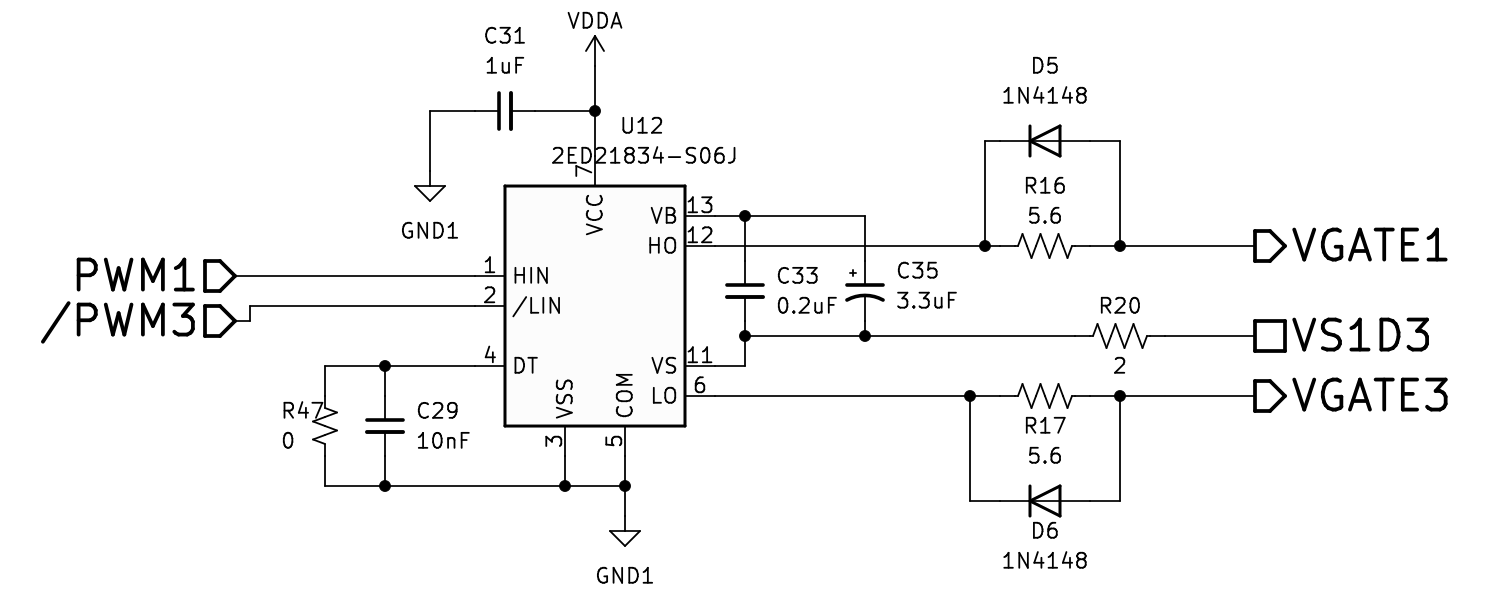
\includegraphics[scale=0.95]{Imagenes/Circuito Driver.png}
    \caption{Circuito de conexión del driver 2ED21834-S06J. El circuito del driver para la otra columna es idéntico.}
    \label{circuito_driver}
\end{figure}

Aquí se puede ver el driver, indicado por la referencia U12, al que le llegan las señales de comando PWM a sus pines HIN y /LIN para el transistor del lado alto y bajo de la columna respectivamente (al estar negada  la entrada para el transistor bajo, la señal que le llega debe estar invertida). Luego, conectado entre el pin DT y tierra se encuentra la resistencia de dead-time, que cuyo valor define el dead-time o tiempo muerto $t_{DT}$. En la salida, se conecta a los pines HO (alto) y LO (bajo) una resistencia limitadora en paralelo con un diodo que permite la descarga de las capacitancias de los transistores, y entre los pines VB y VS se coloca el capacitor que completa el circuito de bootstrap, que se explicará mas adelante. En lo que hace referencia a conexiones a tierra, este circuito, al estar del lado primario del convertidor, se conecta a la referencia $GND_1$.\\

El dimensionamiento de todos estos componentes se va a tratar a continuación siguiendo las recomendaciones del fabricante disponibles en hojas de datos y notas.

\subsubsection{Dimensionamiento de Componentes}

\lipsum[1]\\

\lipsum[2]\\

\subsubsection{Esquema Interno del Dispositivo}

\lipsum[1]\\

\begin{figure}[h]
    \centering
    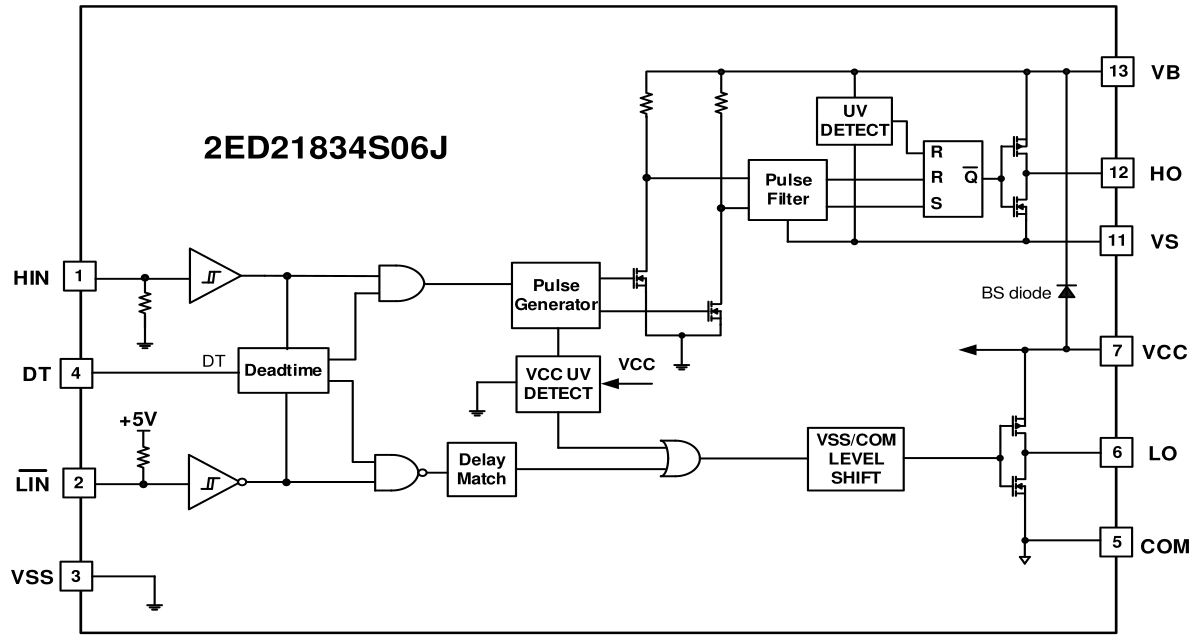
\includegraphics[scale=0.25]{Imagenes/Esquema Interno Driver.png}
    \caption{Diagrama de bloques interno del driver 2ED21834-S06J de Infineon Technologies.}
    \label{interno_driver}
\end{figure}

\lipsum[2]\\

\lipsum[3]\\

\lipsum[4]\\